\documentclass{article}
\usepackage[pdftex]{graphicx}
\usepackage{siunitx}

\usepackage[T2A]{fontenc}
\usepackage[utf8]{inputenc}
\usepackage[bulgarian]{babel}

\begin{document}

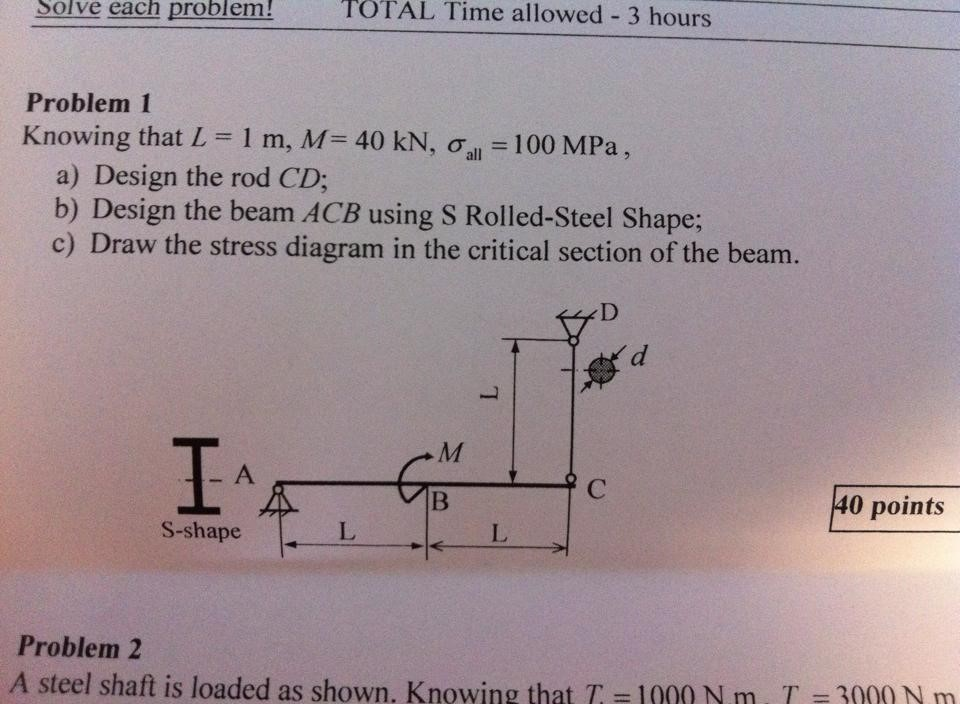
\includegraphics[width=1\textwidth]{images/problem}~

\section{Theory}
Design of beams, subjected to pure bending is explained on page 29-35 in [1].
In particular, we need: \\
$$ S_{min} \geq \frac{M_{max}}{\sigma_{all}} $$
, where: \\
$S_{min}$ - required minimum of the section modolus \\
$M_{max}$ - maximum bending moment \\
$\sigma_{all}$ - allowable stress in the material.
\\
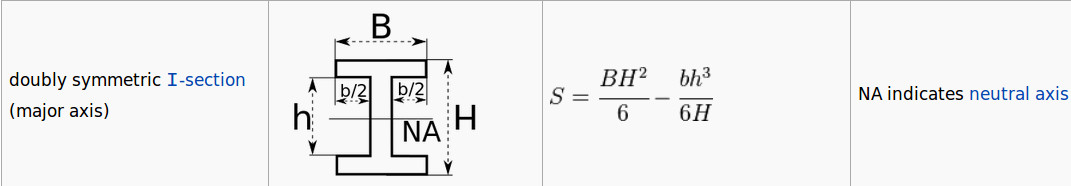
\includegraphics[width=1\textwidth]{images/modulus}~
\\
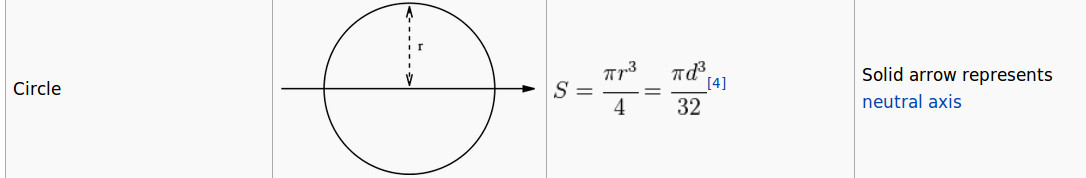
\includegraphics[width=1\textwidth]{images/circle-modulus}~
\\
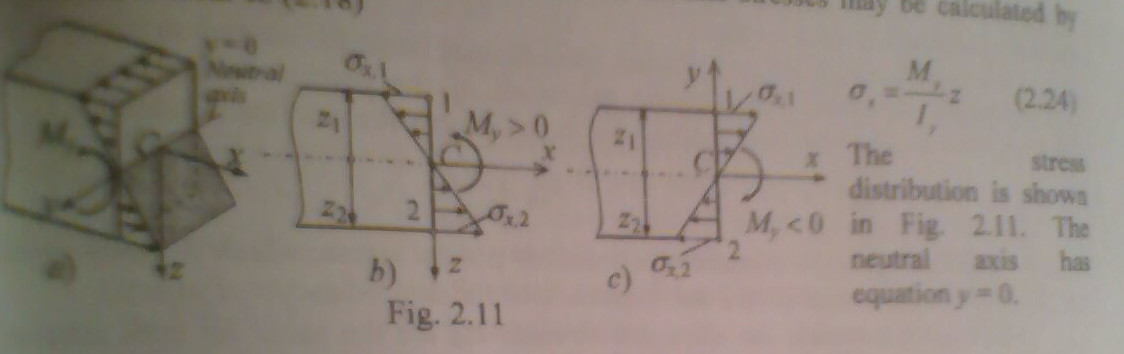
\includegraphics[width=1\textwidth]{images/y-stress}~
\\


\section{Free Body Diagram}
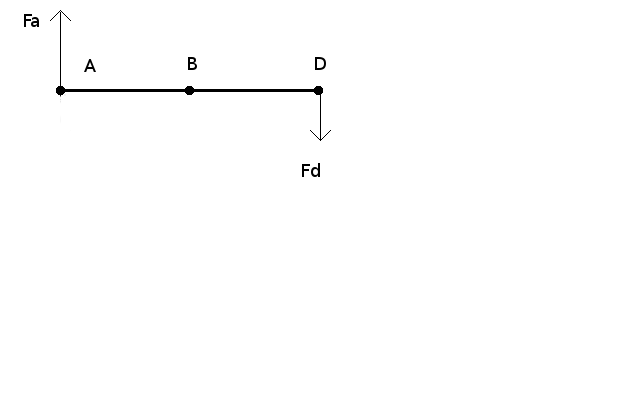
\includegraphics[width=1\textwidth]{images/fbd}~
\\
Support reactions are:
$$ F_A = F_D = M L = 40\si{\kilo\newton\meter} * 1\si{\meter} = 40\si{\kilo\newton} $$

\section{a. Design the rod CD}
Rod section modulus is:
$$ S = \frac{\pi d^3}{32} $$
Equating the stress to the highest allowable, yields the minimum section modulus:
$$ \sigma_{rod} = \frac{F_D}{S_{rod}}  $$
$$ S_{rod, min} = \frac{F_D}{\sigma_{all}} = \frac{40\si{\kilo\newton}}{100\si{\mega\pascal}} = 4 * 10^{-4} \si{\meter}^3 = 400 \si{\centi\meter} 4 * 10^5 \si{\milli\meter}^3$$
$$ d_{min} = \sqrt[3]{\frac{32 S}{\pi}} = 4.07 * 10^{-3} $$
So the rod needs to be about $4\si{\milli\meter}$ in diameter.
For a safety factor of $2$ $d=8mm$ should be a suitable design for the rod.

\section{b. Design the beam ACB using S Rolled-Steel Shape;}
$$ \sigma_x = \frac{M_y}{S_y}z $$
Both the section modolus and the maximum $z$ deviation are variables.
We shall choose a $z_{max}$ value and select a beam with appropriate section modulus ([3], page 13).
$$ S_{y, min}  = \frac{My z_{max}}{\sigma_{all}} = \frac{40\si{\kilo\newton\meter} * (200/2)\si{\milli\meter}}{100\si{\mega\pascal}} = 4 * 10^{-3}\si{\meter}^3 = 4000\si{\centi\meter}^3 $$
This number is too large, nothing i nthe catalogue represents such modulus.

\section{Notice}
Note that the bending moment $M$ is listed in units of $\si{\kilo \newton}$ instead of $\si{\newton\meter}$.
The tet has been read as if the bending moment is $N = 40 \si{\kilo\newton\meter}$

\section{References}
1. Strength of Materials, Georgi Stoychev, 2006, TU-Sofia \\
2. https://en.wikipedia.org/wiki/Section\_modulus \\
3. Таблици по "Съпротивление на материалите", доц. д-р инж. Ленин Лазаров и др., 2007, ТУ-София
\end{document}
